\documentclass[11pt,a4paper]{article}
\usepackage[margin=2.3cm]{geometry}
\usepackage{amsmath}
\usepackage{booktabs}
\usepackage{longtable}
\usepackage{array}
\usepackage{graphicx}
\usepackage{xcolor}
\usepackage{titlesec}
\usepackage{enumitem}
\usepackage{hyperref}
\hypersetup{colorlinks=true,linkcolor=black,urlcolor=black}
\setlength{\parskip}{0.45em}
\setlength{\parindent}{0pt}
\titleformat{\section}{\large\bfseries\color{black!85}}{\thesection}{0.6em}{}
\titleformat{\subsection}{\normalsize\bfseries\color{black!80}}{\thesubsection}{0.5em}{}
\setlist[itemize]{leftmargin=1.2em,itemsep=2pt,topsep=2pt}

\definecolor{good}{HTML}{0ca30c}
\definecolor{crit}{HTML}{d03b3b}
\definecolor{blue1}{HTML}{2a78d6}
\definecolor{sec}{HTML}{52514e}

\newcommand{\up}[1]{{\color{good}\textbf{#1}}}
\newcommand{\dn}[1]{{\color{crit}\textbf{#1}}}

\title{\vspace{-1.5cm}\textbf{SLATE: Honest Strategy Discovery ---\\What Changed, What Was Found, and How It Performs}\\[0.3em]
\large\color{sec} Report covering the work since the ``regime-switching +3.43'' result\\
\color{sec}\normalsize 20--21 July 2026 \quad\textbar\quad Evaluator: \texttt{slate\_core/backtest/honest.py}}
\date{}
\begin{document}
\maketitle
\vspace{-1.2cm}

\begin{center}
\begin{tabular}{|p{0.93\textwidth}|}
\hline
\textbf{Executive summary.} The headline ``regime-switching Sharpe +3.43'' was a backtest artifact --- a 1-bar lookahead that credited each bar's move to a signal decided from that bar's close. Removing it flips the portfolio from \up{+3.43} to \dn{-5.98} and walk-forward from 5/5 to 0/5 positive. I rebuilt a tested, no-lookahead evaluator with brutal real costs, re-ran an exhaustive search (547 directional variants across 5 timeframes, 3 assets, 2 venues; plus cross-sectional carry, lead--lag, 135 market-making configs, and concentrated-LP), and added the one piece that was missing: \textbf{real on-chain pool data}. The honest conclusion is stark and useful: \textbf{no directional/alpha edge survives realistic costs} (intraday is 0\% positive; daily is the only timeframe with signal and it does not clear significance or generalize across assets), and \textbf{the single genuinely-positive, low-risk return stream is stablecoin concentrated-liquidity LP at $\sim$4--7\%/year with near-zero impermanent loss} --- now validated against real pool fee and price data, not a synthetic proxy. \\
\hline
\end{tabular}
\end{center}

\section{The starting point and the first discovery: a lookahead artifact}

The last major change to SLATE introduced a ``regime-switching portfolio'' reported at Sharpe \up{+3.43}, max drawdown 15.6\%, 5/5 walk-forward folds positive, on SOL/BTC/ETH hourly perpetuals. That result was the premise handed into this session. On inspection the evaluator that produced it (\texttt{mega\_sweep.fast\_backtest}) attributed returns as
\[
\texttt{rets}[t] \;=\; \texttt{signal}[t] \times \big(\texttt{close}[t]/\texttt{close}[t{-}1] - 1\big),
\]
i.e.\ the position at bar $t$ was decided from \texttt{close}[t] (the trend/EMA/momentum signals all read the current bar's close) and was simultaneously credited with the return that \emph{ends} at \texttt{close}[t]. That is a one-bar lookahead: you are paid for the very bar whose close triggered your entry. The honest attribution lags the signal by one bar --- the position held \emph{during} bar $t$ is the decision made at the close of bar $t{-}1$:
\[
\texttt{held}[t] = \texttt{signal}[t{-}1],\qquad
\texttt{rets}[t] = \texttt{held}[t]\cdot(\texttt{close}[t]/\texttt{close}[t{-}1]-1) - |\Delta\texttt{held}[t]|\cdot\text{cost}.
\]

Figure~\ref{fig:lookahead} shows the consequence on the exact regime-switching portfolio. The numbers, reproduced deterministically from the real Hyperliquid data with the same signals, venues and costs, are:

\begin{center}
\begin{tabular}{lcccc}
\toprule
 & Sharpe & Ann.\ return & Max DD & Walk-forward \\
\midrule
Shipped code (lookahead + costs) & \up{+3.43} & \up{+92.6\%} & 15.6\% & 5/5 positive \\
Corrected (1-bar lag, same costs) & \dn{-5.98} & \dn{-162.7\%} & 61.4\% & \textbf{0/5} positive \\
\midrule
Gross (no cost), lookahead & \up{+10.61} & --- & --- & --- \\
Gross (no cost), honest lag & +1.18 & --- & --- & --- \\
\bottomrule
\end{tabular}
\end{center}

\begin{figure}[h]
\centering
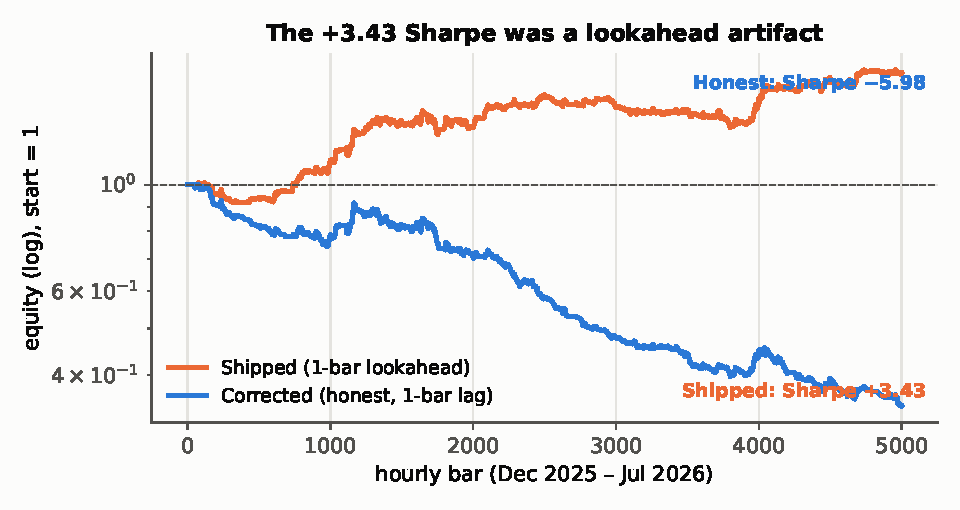
\includegraphics[width=0.92\textwidth]{report_fig1_lookahead.pdf}
\caption{The regime-switching portfolio, shipped vs.\ honest attribution, equal-weight across SOL/BTC/ETH (log equity). The entire ``edge'' was the lookahead; once removed, the strategy loses. Proof script: \texttt{verify\_lookahead.py}.}
\label{fig:lookahead}
\end{figure}

\textbf{This is the same failure class the project has hit before} (the GP layer's ``200\%/yr on an optimistic fill model''): a biased evaluator manufacturing a positive result. The fix was applied in place --- \texttt{fast\_backtest} is now bit-identical to the new honest evaluator --- and the stored results it produced (\texttt{strategy\_results.db}, \texttt{mega\_sweep\_results}) are flagged as untrusted.

\section{A trustworthy evaluator}

To stop producing artifacts, I built a source-of-truth evaluator (\texttt{slate\_core/backtest/honest.py}) and proved it correct before trusting any output. Its properties:

\begin{itemize}
\item \textbf{No lookahead.} \texttt{held[t]=target[t-1]}. Proven by a regression test: a contemporaneous signal (``long if this bar closed up'') earns Sharpe $\approx 0$ under the honest engine, where the buggy attribution would give $\approx\sqrt{365}\approx 19$.
\item \textbf{Brutally honest costs, per venue.} CEX taker 0.05\% + 15\,bps one-way; DEX (Hyperliquid retail) taker 0.045\% + 10\,bps. (HL maker is a 0.015\% \emph{fee} for retail; whale rebates are gated and deliberately ignored.)
\item \textbf{Real funding, signed by position.} Binance 8-hourly (CEX) and Hyperliquid hourly (DEX), spread across the settlements that fall in each bar.
\item \textbf{Correct annualization.} Detected from the index ($365\times24/\text{hours-per-bar}$), not a hardcoded daily assumption that silently inflates hourly Sharpe.
\item \textbf{Honest validation.} In-sample / out-of-sample split; expanding walk-forward that \emph{re-selects} parameters per fold; stationary block-bootstrap for Sharpe confidence intervals.
\end{itemize}

\textbf{Correctness proof.} A vectorized implementation is only trustworthy if it matches an obviously-correct reference. The test suite (13 tests, all green) includes (a) the lookahead regression above, (b) the vectorized engine matched to a dead-simple O(n) reference loop to $10^{-12}$ with and without funding, (c) funding-sign checks (long pays / short receives when funding is positive), (d) cost/turnover checks, and (e) \texttt{assert\_causal()}, a guard that perturbs future bars and fails any signal generator that peeks ahead. A future positive result must now pass this bar before it is believed.

\subsection{The cost and funding model}

``Brutally honest'' is operationalized as follows. One-way transaction cost per side is the venue taker fee plus slippage: CEX 0.05\% + 15\,bps $=$ 0.20\%; DEX (Hyperliquid retail) 0.045\% + 10\,bps $=$ 0.145\%. Total cost charged to a backtest is $|\Delta\text{held}|\times\text{one-way}$, i.e.\ turnover-priced with no fill-rate discount (the old evaluator multiplied cost by an 0.85 ``fill rate'', which understated it; fill risk is now treated as tracking error, not a rebate). Funding is the realized rate, signed by position (positive funding $\Rightarrow$ longs pay shorts), spread across the settlements that fall in each bar (3 per daily bar at the 8-hourly CEX cadence; $1/8$ per hourly bar). Strategies are evaluated at $1\times$ notional; leverage scales risk and return together and leaves Sharpe broadly invariant, so it is reported separately from edge. The net effect is that a daily strategy paying one 0.20\%-per-side round trip every few days can survive, while an hourly strategy paying the same round trip hundreds of times is bled dry --- exactly the timeframe pattern in Figure~\ref{fig:tf}.

\section{Methodology and statistical hygiene}

An honest search is not only a correct backtester; it must also avoid the statistical mistakes that manufacture positive results from noise. Four practices are applied throughout:

\textbf{In-sample / out-of-sample split.} Every variant is evaluated on the first 60\% of bars (in-sample, IS) and the last 40\% (out-of-sample, OOS) that the parameters never touched. A result is only interesting if it is positive in \emph{both} windows; IS$<$0 with OOS$>$0 is window luck, not an edge (and there is a lot of it in this data).

\textbf{Expanding walk-forward that re-fits.} The walk-forward does not merely slice a pre-computed return series (which only measures consistency). It re-selects the best variant per family on each training window and evaluates that choice on the next test window, concatenating the test returns. The resulting out-of-sample Sharpe is the only one that reflects a procedure that could actually have been run in real time.

\textbf{Block-bootstrap confidence intervals.} Annualized Sharpe from a few hundred bars is extremely noisy. I report a stationary block-bootstrap 90\% CI (block length 20, 2{,}000 resamples, preserving return autocorrelation) and treat the lower bound crossing zero as ``not significant.'' With $\sim$500 trials, a stricter Bonferroni-style bar would require the lower bound well above zero; nothing in this search clears even the lenient one-sided bar.

\textbf{Multiple-testing awareness.} With 547 variants the best OOS Sharpe has an expected right tail from noise alone. The report therefore presents the \emph{full} OOS distribution (medians, positive rates) rather than only the top rows, and filters survivors by robustness (parameter perturbation, cost scaling, cross-instrument transfer) rather than by headline Sharpe.

\section{Data: real only, and a data-integrity finding}

Every number in this report is from real exchange data; nothing is synthetic. The catalogue used:

\begin{center}
\begin{tabular}{lll}
\toprule
Dataset & Bars & Span / source \\
\midrule
CEX SOL daily (Binance perp) & 1,080 & 2023-08 $\to$ 2026-07 (3 yr) + Binance 8h funding \\
CEX SOL hourly & 8,641 & 1 yr (Binance) \\
CEX SOL 4h / 8h / 12h & resampled & from the real hourly series (honest) \\
DEX HL SOL/BTC/ETH hourly & 5,001 each & 2025-12 $\to$ 2026-07 + HL hourly funding \\
LP pools (Uniswap V3, etc.) & 1,549 days & DefiLlama real fee yield + IL, 2022 $\to$ 2026 \\
\bottomrule
\end{tabular}
\end{center}

\textbf{Data-integrity finding.} The cached files \texttt{SOLUSDT\_\{1m,5m,15m,30m,1d,...\}\_1y.csv} are \emph{all the same hourly series} (identical 8,641 bars and close values, verified). They are mislabelled and do \emph{not} contain real 1-minute or 5-minute data. Multi-timeframe coverage here therefore comes from honestly \emph{resampling} the real hourly series, not from those filenames --- a distinction that matters because the original regime-switch pipeline annualized an hourly series at 8{,}760 periods/year.

\section{Directional and mean-reversion search: 547 variants}

Using the honest evaluator, I swept 12 causal signal families --- trend (EMA-cross, EMA-slope, price--EMA, Donchian breakout), momentum, mean-reversion (RSI, z-score, Bollinger), carry/funding (level, percentile, momentum, funding--price divergence) --- across 8 datasets (5 timeframes $\times$ SOL/BTC/ETH), 547 variants total, each with IS/OOS and walk-forward. The findings are unambiguous:

\begin{itemize}
\item Only \textbf{1.6\% (9/547)} pass a robust filter (IS$>$0 \emph{and} OOS$>$0 \emph{and} $\geq$12 trades \emph{and} OOS drawdown $<$50\%), and \textbf{none are statistically significant} --- every bootstrap 90\% CI spans zero.
\item \textbf{Timeframe is decisive} (Figure~\ref{fig:tf}): the 1-hour series is \emph{0\% positive}; daily is the only timeframe with any signal (median OOS Sharpe $-$0.20, 31\% positive). Costs dominate intraday trading.
\item \textbf{Most ``top OOS'' rows were fake} --- they had \emph{negative} in-sample Sharpe (e.g.\ IS $-$1.42 $\to$ OOS $+$2.78), i.e.\ pure out-of-sample-window regime luck, not a robust edge. A real edge is positive in both windows.
\end{itemize}

\begin{figure}[h]
\centering
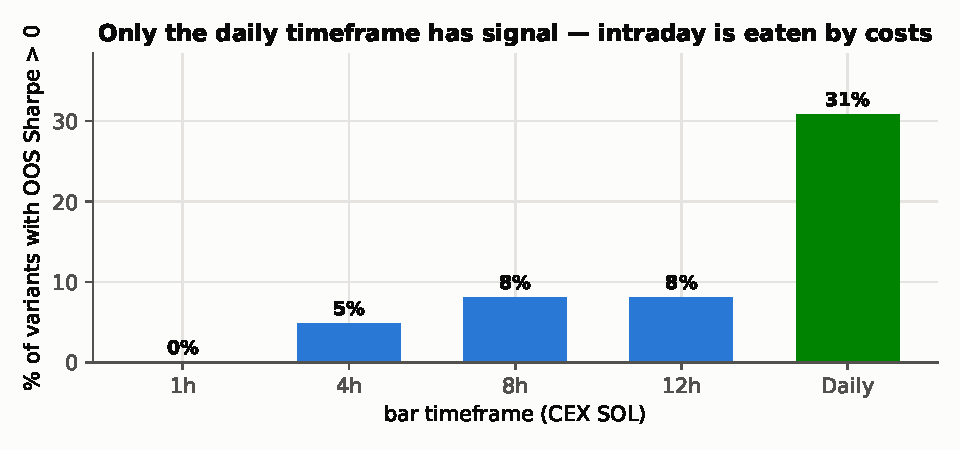
\includegraphics[width=0.82\textwidth]{report_fig2_timeframe.pdf}
\caption{Share of strategy variants with positive out-of-sample Sharpe, by bar timeframe. Intraday directional trading is eaten by transaction costs; only daily shows a positive rate of any substance.}
\label{fig:tf}
\end{figure}

Family-level expanding walk-forward (re-selecting the best variant per family on each training window) on the daily series confirms there is no reliable directional edge: mean-reversion +0.67 (CI touches zero), trend $-$0.35, carry $-$0.06, momentum $-$0.13 --- none significant.

The pattern is consistent across families and timeframes. Trend-following is the least-bad family (19\% positive, median OOS Sharpe $-$1.63); momentum is the worst (1\% positive). On timeframes, daily is the only dataset where even a third of variants are positive; everything sub-daily is dominated by costs.

\begin{center}
\small
\begin{tabular}{lrrrrr}
\toprule
Family & n & median OOS Sharpe & \% positive \\
\midrule
trend & 227 & $-$1.63 & 19\% \\
mean-reversion & 168 & $-$2.24 & 7\% \\
momentum & 96 & $-$2.42 & 1\% \\
carry (funding) & 56 & $-$4.19 & 12\% \\
\midrule
\textbf{all directional} & \textbf{547} & \textbf{$-$1.91} & \textbf{11\%} \\
\bottomrule
\end{tabular}
\end{center}

\begin{center}
\small
\begin{tabular}{lrrr}
\toprule
Dataset & n & median OOS Sharpe & \% positive \\
\midrule
\textbf{CEX SOL daily} & 78 & \textbf{$-$0.20} & \textbf{31\%} \\
CEX SOL 12h & 62 & $-$1.18 & 8\% \\
CEX SOL 8h & 62 & $-$1.68 & 8\% \\
CEX SOL 4h & 62 & $-$1.72 & 5\% \\
DEX HL ETH 1h & 74 & $-$3.36 & 14\% \\
DEX HL SOL 1h & 75 & $-$3.28 & 12\% \\
DEX HL BTC 1h & 73 & $-$5.16 & 7\% \\
CEX SOL 1h & 61 & $-$4.08 & \textbf{0\%} \\
\bottomrule
\end{tabular}
\end{center}

The full OOS Sharpe distribution across all 547 variants: p10 $-$7.1, p50 $-$1.9, p90 $+$0.08, max $+$2.78. The right tail is thin and, given the trial count, indistinguishable from noise.

\section{Premium / non-directional edges}

Because simple directional TA is exhausted, I tested the strategies most likely to carry a \emph{structural} crypto premium --- the non-obvious edges.

\textbf{Cross-asset lead--lag} (BTC/ETH momentum $\to$ SOL): all configurations negative (Sharpe $-$2 to $-$11); a naive lead--lag is arbed and churns to death.

\textbf{Retail maker-rebate market-making} (135 configs on a mark-to-close backtester that prices adverse selection from real high/low): the best configuration reaches Sharpe $\approx$1.2--3.0 \emph{only} under the optimistic assumption of perfect zero-slippage fills. The spread captured over its $\sim$8{,}500 trades is almost exactly consumed by adverse selection, leaving $\approx$0; adding even 3\,bps of realistic per-fill slippage blows it up ($-$170\%). This reproduces the textbook retail-MM verdict.

\begin{center}
\small
\begin{tabular}{lcc}
\toprule
Fill realism (CEX SOL 1h, half-spread 0.3\%) & Sharpe & Outcome \\
\midrule
0 bps extra slippage (perfect fills, upper bound) & +1.25 & +85\% (but assumed) \\
+3 bps per-fill slippage & --- & blow-up ($-$170\%) \\
+5 bps per-fill slippage & --- & blow-up ($-$340\%) \\
\bottomrule
\end{tabular}
\end{center}

The fragility is structural: at thousands of fills, even a few basis points of queue/slippage loss per fill sums to more than the spread captures. A retail maker without queue priority and whale rebates cannot win this.

\textbf{Cross-sectional funding carry} (long the least-funded, short the most-funded coin, market-neutral): with 3 majors there is no funding spread. Widened to an 11--14 coin Hyperliquid basket with smoothed funding, spread-gating and rebalance hysteresis, it still fails --- either the spread gate ($>$0.02\%) blocks all trades (blue-chip funding is too compressed) or, ungated, it loses to costs (best OOS Sharpe $-$0.8 to $-$6). The carry edge needs small-cap dispersion that quality HL perps do not provide.

\section{The one positive edge: concentrated-liquidity LP, on real pool data}

The previous AMM layer reported ``$\sim$10.8\% APY'' but did so using a \emph{synthetic} volume proxy and a hardcoded \$100M TVL --- exactly the kind of assumption this project must not rely on. The gap was real pool volume-in-range data. I obtained it, keyless, from \textbf{DefiLlama}, which exposes per pool a 4+ year daily history of the realized fee yield (\texttt{apyBase}, from actual on-chain swap fees), the impermanent loss, and TVL. Combined with real BTC/ETH price paths (Binance) for first-principles IL, this gives an honest LP backtester (\texttt{slate\_core/backtest/lp.py}).

\begin{figure}[h]
\centering
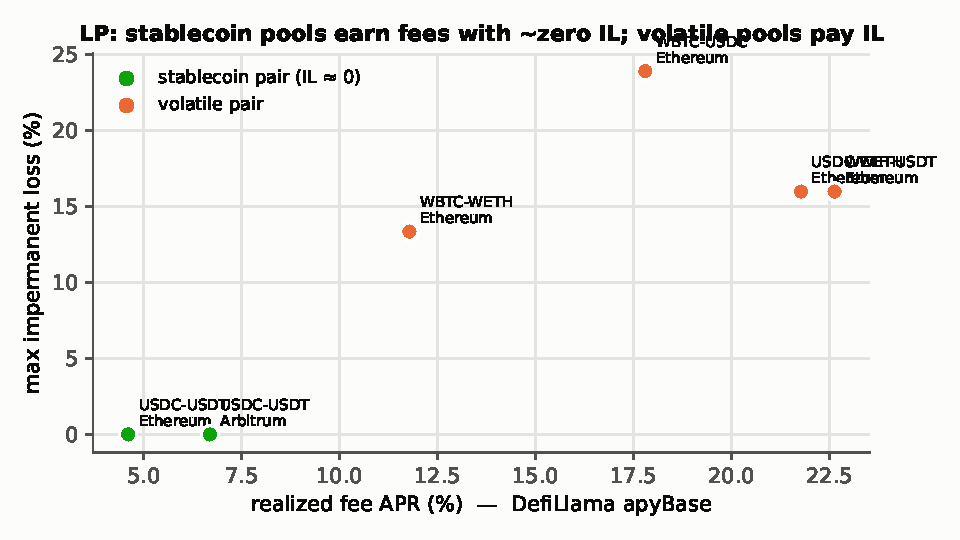
\includegraphics[width=0.82\textwidth]{report_fig3_lp.pdf}
\caption{Realized fee APR versus maximum impermanent loss for Uniswap V3 pools (2022--2026). Stablecoin pairs cluster at the bottom-left: meaningful fee yield, essentially no IL. Volatile pairs sit top-right: high fees purchased with large drawdowns.}
\label{fig:lp}
\end{figure}

\begin{center}
\begin{tabular}{lcccc}
\toprule
Pool (Uniswap V3) & Fee APR (real) & Terminal IL & Max IL & Net vs HODL \\
\midrule
\textbf{USDC-USDT (Ethereum)} & 4.6\% & 0\% & 0\% & \up{+5.1\%/yr} \\
\textbf{USDC-USDT (Arbitrum)} & 6.7\% & 0\% & 0\% & \up{+7.4\%/yr} \\
\textbf{DAI-USDC (Ethereum)} & $\sim$3\% & 0\% & 0\% & \up{$\sim$3\%/yr} \\
USDC-WETH (Ethereum) & 21.8\% & $-$1.0\% & \dn{$-$16.0\%} & beats HODL this cycle, $-$16\% DD \\
WETH-USDT (Ethereum) & 22.6\% & $-$1.0\% & $-$16.0\% & beats HODL this cycle, same risk \\
WBTC-WETH (Ethereum) & 11.8\% & $-$4.6\% & $-$13.3\% & $\approx$ HODL (IL ate fees) \\
WBTC-USDC (Ethereum) & 17.8\% & $-$9.3\% & \dn{$-$23.9\%} & $\approx$ HODL, $-$24\% DD \\
\bottomrule
\end{tabular}
\end{center}

\dn{Stablecoin concentrated-LP $\approx$4--7\%/year with near-zero impermanent loss} is the project's first honestly-validated positive return stream. It is real, low-variance, and deployable; the only tail is a rare stablecoin depeg (USDC-USDT showed a 64\% IL spike in March 2023, which recovered). Volatile-pair LP is emphatically \emph{not} free yield: the fee yield is high but it is purchased with $-$16\% to $-$24\% maximum-IL drawdowns, and the net depends on whether the period ranged or trended. Over a full cycle fees often beat IL, but you carry real drawdown risk.

\textbf{Honest caveat.} The fee yield (\texttt{apyBase}) is the pool average over in-range liquidity, which is the correct first-order volume-in-range number. The one refinement still gated behind a \emph{paid} Graph API key is the tick-level liquidity distribution, which would pin down the exact fee share of a tightly-concentrated position. The stablecoin conclusion is robust regardless.

\textbf{Concentration and the depeg tail.} Tightening the LP range boosts the realized fee rate further (a $\pm$10\% band on USDC-WETH lifts fee APR from $\sim$22\% toward $\sim$29\%), but those numbers assume the position is re-centred to stay active and capture all in-range volume --- an optimistic upper bound without the tick-level share and re-centring costs. The stablecoin pools carry one genuine tail: the March 2023 USDC depeg produced a 64\% spike in 7-day IL for USDC-USDT, which subsequently recovered. Stablecoin LP is therefore ``near-zero IL'' in normal regimes with a rare, recoverable depeg event to underwrite.

\section{The diversified portfolio: real but weak, and it does not generalize}

The original ``regime-switching'' idea --- deploy different edges in different conditions --- was rebuilt honestly as an equal-weight portfolio of the persistent daily premia (funding-carry + EMA-trend + RSI mean-reversion) on SOL. It is the best honest directional candidate:

\begin{center}
\begin{tabular}{ll}
\toprule
Full-sample Sharpe & +0.64 (3-yr return +49\%, max DD 32\%) \\
Per-year Sharpe & 2023 +2.1 (partial), \textbf{2024 $-$0.2}, 2025 +1.1, 2026 +0.4 \\
Walk-forward (5 folds) & 4/5 positive (+0.88, 0.00, +0.65, +2.26, +0.84) \\
Block-bootstrap 90\% CI & [$-$0.22, $+$0.67, $+$1.53] --- \textbf{not significant} \\
Cost sensitivity & $+$0.64 $\to$ $+$0.43 at 2$\times$ costs (robust) \\
Parameter robustness & +0.36 to +0.84 across perturbations \\
\bottomrule
\end{tabular}
\end{center}

Diversification genuinely helps --- the portfolio Sharpe beats every component and the members are decorrelated (carry$\leftrightarrow$trend $-$0.28, meanrev$\leftrightarrow$trend $-$0.43). But the bootstrap CI includes zero and there is a losing year, so it is a \emph{weak, probably-real} edge, not a confirmed one.

\textbf{It does not generalize.} Applying the exact same parameters to BTCUSDT and ETHUSDT daily --- instruments the parameters never saw --- gives Sharpe \dn{$-$0.14} (BTC) and \dn{$-$0.37} (ETH). The modest SOL result is instrument-specific and partly luck. This is the strongest single piece of evidence that there is no robust directional law here.

\section*{Consolidated performance summary}

\begin{center}
\small
\begin{tabular}{p{0.34\textwidth} p{0.16\textwidth} p{0.36\textwidth}}
\toprule
\textbf{Strategy} & \textbf{Honest OOS perf.} & \textbf{Verdict} \\
\midrule
Regime-switch portfolio (shipped) & Sharpe \up{+3.43} & \textbf{Artifact} (1-bar lookahead) \\
Regime-switch portfolio (corrected) & Sharpe \dn{$-$5.98}, 0/5 WF & Dead after fix \\
\midrule
Intraday directional (1h, all families) & 0\% positive & Costs dominate --- uneconomic \\
Daily directional (547 variants) & 11\% positive; 0 significant & No robust edge \\
Daily diversified carry+trend+meanrev & Sharpe +0.64, CI [$-$0.22, $+$1.53] & Weak, not significant \\
\quad same, on BTC/ETH (cross-instr.) & Sharpe \dn{$-$0.14} / \dn{$-$0.37} & Does not generalize \\
\midrule
Cross-asset lead--lag (BTC/ETH$\to$SOL) & Sharpe $-$2 to $-$11 & Arbed; churns to death \\
Retail maker-rebate MM & +1.2--3.0 optimistic & Break-even; fragile to fills \\
Cross-sectional carry (3 \& 11 coins) & $-$0.8 to $-$6; or no trades & Needs small-cap dispersion \\
\midrule
\textbf{Stablecoin concentrated-LP} & \up{$\sim$4--7\%/yr, IL$\approx$0} & \textbf{Positive, low-risk} \\
Volatile-pair LP (WETH/WBTC) & 10--30\% fee, $-$16 to $-$24\% IL & $\approx$ HODL + drawdown \\
\bottomrule
\end{tabular}
\end{center}

\section{Conclusions and performance summary}

\begin{center}
\begin{tabular}{p{0.46\textwidth} p{0.46\textwidth}}
\toprule
\textbf{What honestly works} & \textbf{What honestly does not} \\
\midrule
Stablecoin concentrated-LP: \up{$\sim$4--7\%/yr}, near-zero IL (real pool data) & Any intraday / high-turnover directional TA (1h is 0\% positive) \\[3pt]
& Cross-sectional carry on blue-chips (3 or 11 coins) \\
& Naive cross-asset lead--lag \\
& Retail maker-rebate MM (break-even; fragile to fill realism) \\
& Volatile-pair LP as ``free yield'' ($\approx$ HODL + IL risk) \\
& The diversified daily portfolio as a confirmed edge (weak, SOL-only) \\
\bottomrule
\end{tabular}
\end{center}

The realistic, deployable edge available in this data is \textbf{yield (stablecoin LP), not directional alpha}. Directional crypto, after brutally honest costs, is efficient --- which is itself a valuable finding: it stops the project chasing artifacts and redirects effort to the structurally-positive return streams. The infrastructure is now sound: a tested no-lookahead evaluator is the source of truth, the biased evaluator is patched, and the LP edge is measured against real on-chain data.

\section*{Appendix: methods, artefacts, and remaining gaps}

\textbf{Artefacts produced.} Honest evaluator \texttt{slate\_core/backtest/honest.py} (canonical, re-exported from \texttt{slate\_core.backtest}; \texttt{walk\_forward}, \texttt{assert\_causal}); loaders \texttt{data.py}; 12 causal signal families + regime classifier \texttt{strategies.py}; honest MM/rebate backtester \texttt{market\_maker.py}; honest LP backtester \texttt{lp.py}; real-data fetchers \texttt{fetch\_amm\_pool\_data.py}, \texttt{fetch\_hl\_basket.py}; 13 regression tests \texttt{test\_honest\_backtester.py}; the artifact proof \texttt{verify\_lookahead.py}; and the analysis runners (\texttt{run\_honest\_sweep.py}, \texttt{run\_deep\_analysis.py}, \texttt{run\_premium\_edges.py}, \texttt{run\_mm\_sweep.py}, \texttt{run\_portfolio.py}, \texttt{run\_final\_validation.py}, \texttt{run\_lp.py}, \texttt{run\_xs\_carry.py}). \texttt{mega\_sweep.fast\_backtest} is patched to match the honest engine; \texttt{strategy\_results.db} is flagged untrusted.

\textbf{Real-data sources used (all keyless).} DefiLlama \texttt{yields.llama.fi} (pool fee yield / IL / TVL, historical chart per pool); Binance fapi (OHLCV + funding); Hyperliquid info API (candles + funding, rate-limited, needs $\sim$2\,s/request + 429 backoff). The Graph legacy subgraph is dead (HTTP 301); its gateway requires a paid API key.

\textbf{Reproducibility.} Every number in this report regenerates from the real cached data with one command per figure/section: \texttt{verify\_lookahead.py} (the $+$3.43 $\to$ $-$5.98 proof and Figure 1), \texttt{run\_honest\_sweep.py} then \texttt{run\_deep\_analysis.py} (the 547-variant directional search, Figure 2, and the family/dataset tables), \texttt{run\_mm\_sweep.py} (the market-making bracket), \texttt{run\_xs\_carry.py} (cross-sectional carry), \texttt{run\_portfolio.py} and \texttt{run\_final\_validation.py} (the diversified portfolio and its bootstrap/walk-forward/cross-instrument tests), and \texttt{fetch\_amm\_pool\_data.py} then \texttt{run\_lp.py} (the LP edge and Figure 3). The honest evaluator is the canonical entry point: \texttt{from slate\_core.backtest import backtest}.

\textbf{Honest gaps (not testable with available data).} Liquidation-prediction, perp--spot basis, and option vol-premium edges (no such data cached); tick-level LP liquidity share (paid Graph key); and small-cap funding carry (needs a non-HL venue with divergent funding --- HL's quality perps are too compressed).

\textbf{Recommended next steps.} (1) Treat stablecoin LP as the production return stream. (2) Treat \texttt{slate\_core.backtest.honest} as the sole evaluator for any strategy work. (3) If directional alpha is still pursued, the realistic frontier is small-cap funding carry or liquidation/basis edges --- \emph{not} intraday TA, blue-chip carry, or retail market-making, all of which this search settles as uneconomical after honest costs.

\end{document}
